\newpage
\subsubsection{Turbot Fish}
Wie auch bei den vorherigen \textit{Single Digit Patterns} wird auch beim \textit{Turbot Fish} nur eine Ziffer betrachtet. Gesucht wird eine Kette, die vier Ziffern lang ist, so dass Anfang und Ende eines Kettenglieds in einer gemeinsamen Figur liegen. Wichtig ist dabei, dass im ersten und dritten gemeinsamen Figur die beiden betrachteten Kandidaten die einzigen verbliebenen  sind. Da die Kette vier Glieder lang ist, muss entweder der Anfang oder das Ende der Kette wahr sein, daher können die Kandidaten gelöscht werden, die von beiden Feldern ausgeschlossen werden.

\begin{figure}[h]
\begin{center}
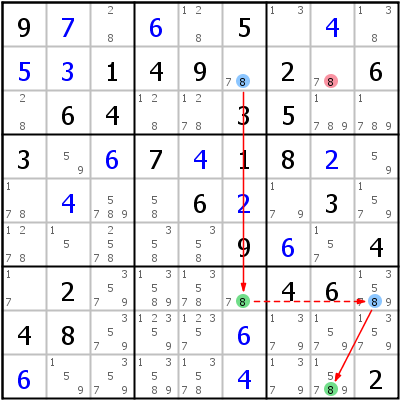
\includegraphics{./img/turbot_fish.png}
\caption{Turbot Fish}
\end{center}
\end{figure}

In der obigen \textbf{Abbildung 3.11} beginnt die Kette der Ziffer 8 im Feld z2s6. In der selben Spalte befindet sich die zweite Ziffer in z7s6, sie ist dort der einzige weitere Kandidat der Ziffer 8, was Voraussetzung für den Turbot Fish ist, da es sich hier um das erste Glied handelt. Die nächste Ziffer liegt in der gleichen Zeile, z7s9. Die letzte Ziffer befindet sich im selben Block wie auch ihr Vorgänger, in z9s8, und auch sie ist hier der einzige weitere Kandidat für diese Ziffer. Wir betrachten zwei Fälle: die Ziffer 8 steht in z2s6 oder sie steht dort nicht. Im ersten Fall kann der rot markierte Kandidat in z2s8 gelöscht werden, da er direkt ausgeschlossen wird. Wenn die 8 dort nicht steht, dann muss sie in z7s6 stehen, da das der einzige andere Kandidat in der Zeile ist. Darum kann die 8 dann nicht in z7s9 stehen. Daraus folgt, dass sie in z9s8 stehen muss, was dann im zweiten Fall die Ziffer 8 in z2s8 ausschließt, womit diese dort in jedem Fall nicht stehen kann.